% This is "sig-alternate.tex" V2.0 May 2012
% This file should be compiled with V2.5 of "sig-alternate.cls" May 2012
%
% This example file demonstrates the use of the 'sig-alternate.cls'
% V2.5 LaTeX2e document class file. It is for those submitting
% articles to ACM Conference Proceedings WHO DO NOT WISH TO
% STRICTLY ADHERE TO THE SIGS (PUBS-BOARD-ENDORSED) STYLE.
% The 'sig-alternate.cls' file will produce a similar-looking,
% albeit, 'tighter' paper resulting in, invariably, fewer pages.
%
% ----------------------------------------------------------------------------------------------------------------
% This .tex file (and associated .cls V2.5) produces:
%       1) The Permission Statement
%       2) The Conference (location) Info information
%       3) The Copyright Line with ACM data
%       4) NO page numbers
%
% as against the acm_proc_article-sp.cls file which
% DOES NOT produce 1) thru' 3) above.
%
% Using 'sig-alternate.cls' you have control, however, from within
% the source .tex file, over both the CopyrightYear
% (defaulted to 200X) and the ACM Copyright Data
% (defaulted to X-XXXXX-XX-X/XX/XX).
% e.g.
% \CopyrightYear{2007} will cause 2007 to appear in the copyright line.
% \crdata{0-12345-67-8/90/12} will cause 0-12345-67-8/90/12 to appear in the copyright line.
%
% ---------------------------------------------------------------------------------------------------------------
% This .tex source is an example which *does* use
% the .bib file (from which the .bbl file % is produced).
% REMEMBER HOWEVER: After having produced the .bbl file,
% and prior to final submission, you *NEED* to 'insert'
% your .bbl file into your source .tex file so as to provide
% ONE 'self-contained' source file.
%
% ================= IF YOU HAVE QUESTIONS =======================
% Questions regarding the SIGS styles, SIGS policies and
% procedures, Conferences etc. should be sent to
% Adrienne Griscti (griscti@acm.org)
%
% Technical questions _only_ to
% Gerald Murray (murray@hq.acm.org)
% ===============================================================
%
% For tracking purposes - this is V2.0 - May 2012

\documentclass{sig-alternate}
\usepackage{color}
\usepackage[usenames,dvipsnames]{xcolor}
\usepackage{url}

\newcommand{\TODO}[1]{{\color{red} TODO: #1}}
\newcommand{\gametitle}{{\color{RoyalPurple} Dragon Architect Academy}}

\toappear{Submitted for review.}

\begin{document}
%
% --- Author Metadata here ---
%\conferenceinfo{Foundations of Digital Games (FDG)}{2015}
% \pdfinfo{
% /Title ()
% /Author (Aaron Bauer, Eric Butler, Zoran Popovic) 
% /Subject ()
% /Keywords ()
% }
%\CopyrightYear{2007} % Allows default copyright year (20XX) to be over-ridden - IF NEED BE.
%\crdata{0-12345-67-8/90/01}  % Allows default copyright data (0-89791-88-6/97/05) to be over-ridden - IF NEED BE.
% --- End of Author Metadata ---

\title{Visual Programming and Cube-Coding Gooooodtimes}

\numberofauthors{1}
\author{Anonymized}

% \numberofauthors{1} 
% \author{
% \alignauthor
% Aaron Bauer, Eric Butler, Zoran Popovi\'c\\
%        \affaddr{Center for Game Science}\\
%        \affaddr{Computer Science \& Engineering}\\
%        \affaddr{University of Washington}\\
%        \affaddr{Seattle, WA 98195}
%        \email{\{awb, edbutler\}@cs.washington.edu}
% }

\maketitle
\begin{abstract}

    \TODO{Giant wall of text just to fill in the space and get an idea of how long the paper actually is. In this paper we present \gametitle{} which is trying to do some interesting research in CS education. CS education is hard, and also a popular thing to do. Attempts for CS stuff/games usually either approach is as a sequence of challanges/puzzles or a free-for-all sandbox funland. We want to explore combining these two aspects. Our contributions include presenting \gametitle{}, thoroughly describing the unaddressed research problems the space, discussing design challenges encountered attempting to tacke these problems, and initial feedback from players.}
\end{abstract}

% A category with the (minimum) three required fields
\category{K.3.2}{Computers and Education}{Computer and Information Science Education -- Computer science education}

\terms{Design, Human Factors}

\keywords{Game-based learning; computational thinking; programming education}

\section{Introduction}
The past few years have seen many efforts to broaden the reach of computer science education and make it available, and appealing, to more students in more places. 
Many of these projects, such as Scratch~\cite{scratch} and Code.org's Hour of Code~\cite{codedotorg}, are educational programming environments that expose users to basic programming concepts. 
Despite the proliferation of these systems, little work has investigated how to design the structure or content of such systems. There have been surveys of both the systems themselves~\cite{guzdial2004programming, kelleher2005lowering} and of research involving these systems~\cite{salleh2013analysis}. Researchers have enumerated desirable properties for such systems~\cite{repenning2010scalable} discussed their design~\cite{powers2006tools}.
Comparative studies of effective ways to present computer science concepts in these systems, however, have been largely absent. 

As the expansion of computer science education, especially for primary and secondary-school students, gathers steam, it would be valuable to have concrete data to guide the development of the educational systems involved. 
This includes the structure of the systems themselves in addition to the curricula and pedagogy they employ. 
This paper focuses on a connected set of research questions that follow naturally from this need.

%How can we effectively teach high-level programming concepts and skills through educational software and games?
%For example, \emph{computational thinking}~\cite{wing2008computational} is a central element of the discussion on programming education.
%There is significant interest in bringing computational thinking into the classroom~\cite{barr2011bringing, lye2014review}, and more research is required on teaching computational thinking skills through educational software and games.
%Another important aspect of teaching programming tools is choice of programming language.
%How does the design of the programming language a system uses affect its users?
%One part of investigating how to teach such skills involes exploring how to teach the strategies and metastrategies, such as divide and conquer, involved in computational thinking.
%Answering such research questions requires exploring the structure of educational games.
%The structure of existing educational programming environments generally falls into one of two groups: (1) an open-ended setting with little to no direct guidance where players are intended to learn via exploration and from instructors or other members of the social community using the system or (2) a linear series of puzzles or exercises with substantial direct guidance, but little in the way of exploration of social interaction. 

Computational thinking is often discussed in the context of educational programming environments and there needs to be more research on how such systems can effectively teach these ideas. 
Programming language semantics are one understudied aspect of this. 
How does the design of the programming language a system uses affect its users' understanding of computational thinking?
Further research should also explore ways to directly teach the strategies and metastrategies, such as divide and conquer, involved in computational thinking instead of expecting learners to absorb them as a result of working with other computer science concepts.
The structure of existing educational programming environments generally falls into one of two groups: (1) an open-ended setting with little to no direct guidance where players are intended to learn via exploration and from instructors or other members of the social community using the system or (2) a linear series of puzzles or exercises with substantial direct guidance, but little in the way of exploration of social interaction. 
Given the limitations inherent to each group, there needs to be an exploration of the design space between these two approaches in which exploration, social community, and some form of direct guidance are integrated together. 

In this paper we present \gametitle{}, an educational game designed to be a tool with which to investigate these questions. 
In our game, players use a visual, drag-and-drop programming language to control a dragon in a 3D grid world. 
The remainder of this paper is as follows: after it describes our game in more detail, it discusses our research goals and how they affected the design of \gametitle{}. 
The paper then gives an overview of players' response to our game and highlights several design issues that have arisen during its development.
The paper concludes with our thoughts on other interesting questions our game might be used to help answer.

\begin{figure*}[t!]
  \centering
  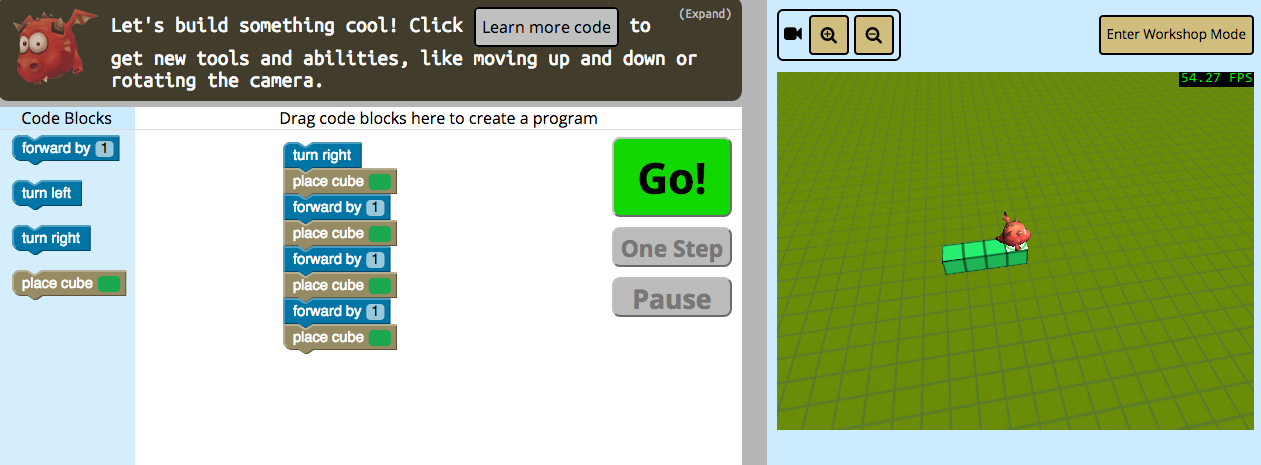
\includegraphics[width=\textwidth]{images/overall-example}
  \caption{The player assembles code for the dragon on the left side, and the dragon and world it inhabits are visualized on the right side. Only a few different code blocks are available to the player initially.}
  \label{fig:overall}
\end{figure*}

\section{\gametitle{}}
\TODO{Can't use macros in section titles because the formatted gets messed up, replace once we choose a title} 
We have been developing \gametitle{} since spring 2014. 
It can be played in a web browser, and similar to many other such systems, the page is separated into two parts: an area where the player can assemble their code and a visualization of the environment their code affects (see Figure~\ref{fig:overall}). 
The visualization uses the Unity game engine~\cite{unity} and the drag-and-drop programming UI is provided by the Blockly library~\cite{blockly}.

The visual language players use is a set of \emph{code blocks} that snap together to form programs. 
The player can move the dragon in three dimensions and have the dragon place and remove cubes of various colors. 
In addition to blocks that control the dragon directly, players can also make use of definite loops and procedures (see Figure~\ref{fig:toolbox}).
Given that syntax can be an obstacle for those new to programming~\cite{stefik2013syntax}, we chose to use a visual language as there is evidence visual languages are helpful to novices~\cite{whitley1997visual}.

As players progress through the game, they alternate between short sequences of puzzles with a specific goal and a specific set of available code blocks and an open-ended sandbox. 
The game begins with puzzles that introduce the idea of assembling and running code, as well as the code blocks for moving the dragon in 2D and putting down cubes.
After that, the player can experiment and build in the sandbox and complete other puzzle sequences to make more code blocks available, switching between sandbox and puzzles at any time. 
In this way, the language the player uses to write instructions for the dragon gradually expands as the player advances.

The popularity and broad appeal of Minecraft~\cite{minecraft} motivated our use of a 3D grid world in which the player's programs could place cubes.
This choice also makes it natural to extend our game in the future with exploration, more complex interaction with the environment, or players working together in a shared world.
Our playtests with \gametitle{} have shown the premise of programming a dragon in a Minecraft-like world appeals to younger players of all genders.
Common sandbox activities have included making the dragon travel very long distances, building big and impressive towers, and spelling one's name out of cubes.

\begin{figure}[htb]
  \centering
  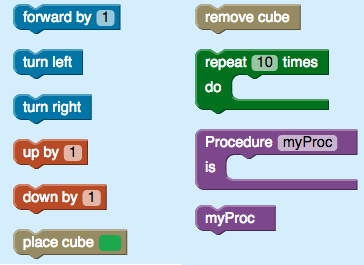
\includegraphics[width=\columnwidth]{images/toolbox-wide}
  \caption{The programming elements available in \gametitle{}.}
  \label{fig:toolbox}
\end{figure}


\section{Research Questions}
\label{sec:research}

Our primary goal for \gametitle{} is to investigate questions in computer science education and game-based learning. 
Specially, we are interested in exploring how to teach compuational thinking skills and problem-solving stategies, and we are interested in exploring which programming languages best support novices in learning these skills. 
This naturally leads to research questions on how an effective educational game should be structured.
Open-ended games and systems typically peform poorly at teaching complex concepts without instructors or other outside help, but linear, direct-guidance based games and systems don't offer the engaging creative and social experiences that can be found in more open-ended settings.
In this section, we describe these research poblems in detail and design decisions informed by these problems.

\subsection{Teaching Computer Science}

\subsubsection{Compuational Thinking}

% what is it
A major goal of our project is to explore methods of teaching \emph{computational thinking}~\cite{wing2008computational} skills.
Many have studied how to increase presence and effectiveness of computational thinking in computer science education (and education in general)~\cite{barr2011bringing, lye2014review},
other others have developed games to teach these ideas~\cite{weintrop2013robobuilder, kazimoglu2012serious}. 
Repenning et al.~\cite{repenning2010scalable} suggest six properties a computational thinking tool for K-12 must have in order to achieve systemic impact. 
Evaluating and characterizing the effectiveness of systems that use these (and other) properties is an ongoing research effort.

\gametitle{}'s design is structred to encourage and require use of computational thinking skills.
Like many programming games, we force the player to automate tasks that they are used to performing manually (in this case, the construction of 3d block structures).
As the player sets more sophisticated goals, abstraction becomes important (e.g., abstracting the building of a wall into a procedure) to keep the visual programming feasible. 

% how can we teach it directly?
As we cannot expect players to learn such complex and abstract skills simply by playing in an environment that requires them, we explore how to effectively directly teach computational thinking skills.
One such skill is a core component of computational thinking: the identification and application of problem-solving strategies (such as divide and conquer). 
A great deal of recent education research suggests that ``curricula can model such strategies for students'' and that appropriate guidance, which in many cases consists of the capabilities afforded by a suitable computational environment, can ``enable students to learn to use these strategies independently''~\cite{report2010computational}. 
Mayer and Wittrock~\cite{mayer1996handbook} call attention to the substantial evidence in the education literature for teaching what they call \emph{domain-specific thinking skills} and \emph{metacognitive skills}. 
The former would include the ability to use a strategy like divide and conquer, and the latter would include knowing when and where to employ that strategy. 
In both cases, Mayer and Wittrock describe studies that have shown teaching these skills directly can improve learning and performance. 

% teaching stategies like divide and conquer
Our initial attempt to directly teach divide-and-conquer is to lead the player though a top-down deconstruction of building a large castle.
The player is presented with a single code block that builds an entire castle, but discovers the construction has a number of flaws. 
The following puzzles each decompose some part of the flawed program in order to give the player a chance to repair it. 
For example, to enable the player to give the castle the correct number of walls and towers, the castle code block is split into a tower block and a wall block that the player uses to write a corrected castle procedure, as shown Figure~\ref{fig:decomp}. 
This part of \gametitle{} needs to be expanded and refined before it can be evaluated, but the larger question certainly merits further attention. 

\begin{figure*}[th!]
  \centering
  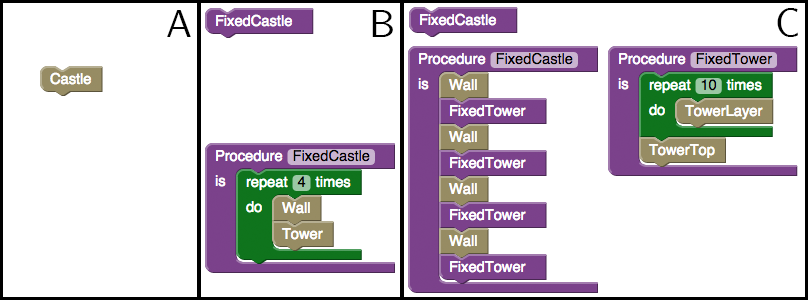
\includegraphics[width=\textwidth]{images/decomp-code}
  \caption{The code required by a progression of levels demonstrating the strategy of divide and conquer. In A, the player uses a single code block to build an entire castle. Then, in B, the player is given an empty FixedCastle procedure, which they must fill with the appropriate number of wall and tower blocks. Finally, in C, the player is given a completed FixedCastle procedure and must fill in the FixedTower procedure as shown.}
  \label{fig:decomp}
\end{figure*}

\subsubsection{Language Semantics for Novices}

For those just starting to program, many aspects of the programming language and programming environment can affect their progress. 
Language syntax and semantics have been extensively studied for professional programmings~\TODO{cite}.
While previous work indicates aspects such as language syntax~\cite{stefik2013syntax}, compiler messages~\cite{nienaltowski2008compiler}, and language semantics~\cite{hoc1990language} can all have an impact, only syntax and compiler messages have been characterized in detail with research on the effectivenss of particular design decisions. 
So while we have drawn on existing research when choosing the programming syntax and input method for players, the literature lacks support for definite conclusions and suggestions for language semantics. 
In addition, we are not aware of any investigation into the relationship between language design and teaching computational thinking.

In order to support research exploration in language semantics, \gametitle{} uses a custom visual programming language instead of using a popular existing language like JavaScript. 
This gives us fine-grained control over how the language behaves, enabling experimentation in language semantics.
Additionally, we do not have to inflict the quirks of any existing language on our players. 
Finally, we have implemented a concrete syntax for our language that corresponds precisely with its visual code-block equivalent, allowing translation to and from concrete syntax, allowing players to choose which method of input they prefer.  
The most apparent drawback of this approach is the lack of existing resources for studets to use.
Using an existing popular language not only comes with a very large and free corpus of learning material, but provides an avenue for students to apply what they have learned directly outside the game.
Possible problems to explore include use of recussion and looping, eager versus lazy evaluation, or type checking.

\subsection{Structure of Learning Environment}

\subsubsection{Guided Discovery Learning}
%Many open-ended creative prgramming tools (such as Scratch) are influenced by \emph{constructionism}, which is a learning theory that proposes students learn effectively by constructing things of social relevance in a social context \cite{kafai06constructionism}.
%One component of constructionism is discovery learning that suggest students learn best by doing and building.
%Others have argued that games are an ideal environment for constructionist teaching \TODO{cite}.
%However, evidence suggests that a purely self-directed learning approach is inadquate for effective learning \TODO{cite}.
%Evidence suggests that pure self-directed discovery learning is not effective in complex domains unless students have prior background knowlege, so these systems often are paired with cirrucla to guide students in use of the system.
%With \gametitle{}, we aim to investigate whether and how structure such as direct guidance and scaffolding can be included in the system itself while preserving the positive aspects of open-ended, social, creative tools.
\TODO{define discovery learning.}
\TODO{define direct guidance.}
\TODO{establish support for guided discovery.}
%Education research indicates that guided discovery, the blending of exploration and direct guidance, can benefit learning when compared to using just one or the other. 
More research is needed on guided discovery learning in games. 

Some games provide a sandbox where players discover the properties of the environment through largely unguided exploration (e.g., Minecraft, SimCity~\TODO{cite}), and others provide a linear sequence of levels designed to teach the player the relevant information (e.g., Portal~\TODO{cite}). 
In terms of learning theory, the former have a lot in common with pure discovery learning (ignoring potential external sources of information such as wikis or friends), while the latter rely on direct guidance. 
Other games teach players by doing something in between. 
Games in the Zelda series~\TODO{cite} contain a non-linear sequence of puzzles and teach new mechanics by requiring the player demonstrate understanding of a new mechanic before they are allowed to progress. 
Strategy games such as Crusader Kings II~\TODO{cite} offer a set of explicit tutorials the player may choose to go through before beginning more open-ended play.
The variety of approaches games take in teaching players leads to interesting questions about how different methods affect what players do in a game, or, in the case of educational software, how they learn. 
Furthermore, for complex topics such as computer science, the concepts a game needs to teach its players are likely to be more difficult to discover through exploration and require more sophisitcation to explain through direct guidance. Thus, more research is needed to refine and evaluate these techniques. 

In the case of \gametitle{}, we have combined structured puzzle levels and an open, unstructured sandbox. 
The puzzles, by leading the player to demonstrate a particular concept, act as a form of direct guidance. 
A process of discovery can then take place in the sandbox where the player is free to experiment with the ideas introduced in the puzzles. 
Our playtesting has shown this to be a promising approach in getting players to understand many of the concepts currently in our game. 

\subsubsection{Social Community}
Another primary aspect of constructionism is that the learning process should occur in a social envionrment in which students are building things that matter to them and the social group.
There are examples where social community has been an important part of the success of an online programming environment. 
Scratch users, for example, have shared millions of projects and even formed online \emph{companies} to tackle projects together~\cite{resnick2009scratch}. 
Research using an online programming environment called MOOSE Crossing~\cite{bruckman1997moose} found that a social context can support and motivate learning programming~\cite{bruckman2000situated}.
This work is supported by research in behavioral and social sciences that indicates sharing and collaboration can improve learning~\cite{bransford2000people}. 
Given these promising results, it is unfortunate the specific contributions of social features to an online programming environment (and how to design those features) remain largely unstudied.

We have incorporated features of this kind into the design of \gametitle{} modeled on the way Scratch lets its users share projects. 
A player can choose to share anything they build in the sandbox, sending it to a gallery containing everyone's shared creations.
Browsing the gallery, players can view, and get the code for, any uploaded construction.
\TODO{we track attribution}

\section{Design Issues}
The design of \gametitle{} has been informed by our research goals, and by existing software such as Minecraft and Scratch. 
In this section we discuss two cases where these objectives presented unusual challenges. 

\subsection{Consistency vs. Experimentation}
Part of Minecraft's popularity is the collaborative multiplayer environment it offers. \TODO{citation, or argument that this is true}
On a Minecraft server, players can explore and shape the world together. \TODO{citation?} 
We want \gametitle{} to be able to provide the same kind of experience, which means giving the world the players inhabit consistency. 
We envision players visiting and admiring each other's constructions or working together on the project. 
While this is relatively straightforward in Minecraft (the whole world shares the same real-time simulation and players' actions are fine-grained with permanent effects), it is complicated in our game by the fact that player input is code. 
Running a single program can have large effects only reversible by tedious effort, so it's important for players to be able to experiment with and tweak their code before committing to it. 
On the other hand, if a player can undo the effects of their programs at will, interactions with existing creations become unpredictable and inconsistent. 

We have so far only partly resolved this tension in \gametitle{}. 
The sandbox makes the effects of programs permanent by default, including any cubes placed and the dragon's position.
To allow for experimentation, the player has the option to switch to \emph{workshop mode}, which resets the world to its previous state each time the player runs a new program. 
The player can freely toggle between these two modes, testing out each program before committing to its results. 
Aside from the fact that the existence of these two modes is difficult to communicate to the player, and that the distinction between them can be confusing, this solution doesn't resolve how to model or visualize the modes in a multiplayer setting. 
Ideally, the player would receive clear indication that effects executed in workshop mode cannot be depended upon.

\subsection{Puzzles as Guidance}
Using puzzles as the guidance in \gametitle{}'s guided discovery is central to the design of the game. 
The puzzles must strike a difficult balance: get the player to the sandbox where they can experiment with their new tools as quickly as possible and support the player in the gradual acquisition of new knowledge and skills. 
Puzzle sequences need to be relatively short to avoid provoking frustration from players who are not engaged by solving puzzles. 

\TODO{this is a super rough idea dump}

The ideal situation is an open sandbox where just-in-time guidance is given at the most appropriate minute, as an effective human tutor would do.
Intelligent tutoring systems accomplish this by modeling tracking player knowledge and skill.
As we do not have a model for our game domain, this is not an option.

Our current approach is to allow the player unlimited usage of the sandbox and programming tools that they have already used.
In order to unlock new programming tools, player must volunteer to start a new puzzle that will directly guide them in some concept.
A list of available modules advertise what techniques and tools players can learn from puzzles.

In tests, players have gotten \emph{stuck} at the sandbox, unsure of what they should do next, or trying to come up with an idea of what to build. 
We need to more clearly communicate the available options, and provide players ideas to get started with and to use as \emph{jumping off points}.
Other players can also be a source of guidance and ideas, so the social features will play an important role in this as well.

However, this approach has several shortcomings.
Emperically in play tests, players have expressed that they wish certain features were available, such as moving the dragon up and down.
In fact, such features were advertised explicitly in the list of modules, but players did not think to check the list, even if they had been there previously.
But even assuming we could get players in the habit of consulting this list, the items they want at the moment was not be obviously on the list.
Perhaps what they do not know how to clearly articulate what the want to do or we as designers have not chosen the best language to describe a techinque.
Then players will not find their desired item on the list.
Human tutors, on the other hand, could help with this translation.

Another problem with this approach is the difficulty in choosing an appropriate sequence of puzzles.
One goal is that players can learn whatever strategy than need to when they need it, with no articifial restrictions gating content.
A contradictory goal is that players are not overwhelmed with concepts at the beginning, as they are in Scratch~\cite{resnick2009scratch} and other fully open tools.
This goal suggest we impose a partial ordering on content and introduce concepts in a deliberate order.
However, with such gating, players may think a feature doesn't exist when, in reality, it's hidden behind several prerequisite concepts.

A potential approach to balance these goals is to expose the entire list of strategies at the start, but still require players to go through the prerequisits.
That is, a player can identify a learning module the wish to reach, and the game will walk them through all the basic skills that they need to get there \TODO{some citation on this style of self-directed learning must exist}.
However, with the entire list was available at the start, seaching for concepts and strategies becomes a more difficult task.

We have also noted that building structures in the sandbox is not necessarily the activity of choice for every player. 
Some choose to \emph{doodle} in the sandbox, scattering cubes, often of different colors, in lines and clusters without trying to assemble anything in particular.
Others exclusively seek out the game's puzzles, more interesting in solving those than working in the sandbox.
We believe the freedom a player has to choose what activity interests them most, and to freely switch between them, allows \gametitle{} to engage a wider range of players.

\subsection{Mental Model Problems}

Conceptually, the most common stumbling block we've observed has been a flawed mental model of how the code relates to what the dragon does. 
For example, a player is doing a puzzle where they need to make the dragon move two spaces forward. 
The current program moves the dragon one space forward. 
After running the code, the player sees that the dragon is now only one space away from the goal. 
They quickly reset the program and run it again, not realizing that this resets the dragon as well. 
Another manifestation of this is players add additional code blocks to an existing program, expecting only the new instructions to be run. 
They are surprised when all the code they have assembled is executed. 
Another frequent, if unsurprising, difficulty is procedures. 
Players often don't understand the separation of a procedure into a definition and zero or more invocations. 
This leads to mistakes such as defining a procedure multiple times in order to use it multiple times, or unintentionally introducing recursive calls. 

\section{Related Work}

\subsection{Educational Technology and Games for Computer Science}

The development of tools designed to teach novices programming dates back to sytems such as Pappert's LOGO~\cite{papert80mindstorms}.
Kelleher and Pausch review programming environments for novices and describe a taxonomy of these systems~\cite{kelleher2005lowering}.
Within that taxonomy, \gametitle{} fist best as a teaching system that targets \emph{structuring programs} and aims to provide learning support both through \emph{social learning} and \emph{providing a motivating context}.

\subsubsection{Open-Ended Creative Systems}
These early tools and some popular tools today are structure as open-ended creative environments.
LOGO allowed players to create drawings by controlling a robot with a virtual pen.
A popular modern example is Scratch~\cite{maloney2010scratch}, a visual programming environment focused on empowering its users to create interactive digital media such as stories and games.
Scratch has been successful in building vibrant community around its open-ended, creative, social environment with millions of projects shared via its website~\cite{scratch}.
 
\TODO{cite and talk about AgentSheets~\cite{repenning2000agentsheets}, Kodu~\cite{maclaurin2009kodu}, Alice~\cite{cooper2000alice}}

\subsubsection{Structured Learning Systems}
Another type of programming educational system is instead arranged as a linear sequence of problems or puzzles.
Step-by-step lessons are available from Khan Academy~\cite{khanacademy} and Codecademy~\cite{codecademy}, in which users program in a popular industry programming language such as Javascript or Java, sometimes with accompanying video.
Code.org~\cite{codedotorg} is a sequence of videos and puzzles where users control characters from popular games like Rovio's \emph{Angry Birds} or movies like Disney's \emph{Frozen} with drag-and-drop programming (like Scratch).

Several games also fall into this category.
The game \emph{LightBot}~\cite{lightbot} asks players to use programming to control a robot in a sequence of linear puzzles.
The game has been used to study education in computational thinking~\cite{Gouws13Lightbot}, and is now featured in Code.org's Hour of Code\footnote{\url{http://lightbot.com/hocflash.html}}.
In \emph{CodeSpells}~\cite{esper2013codespells}, players write Java code to cast spells that control their environment in an adventure game.
In \emph{RoboBuilder}~\cite{weintrop2012robobuilder}, players program robots to battle against enemies.
\emph{BOTS} is a programming puzzle game. The stated goal of the project is to study how community-authored content is used in educational games~\cite{hickspart14}, and it has also been used to explore hint generation~\cite{peddycord14generating}.
We wish to combine direct lessons and open-ended structure into a single system, and explore the tradeoffs and whether we can get advangates from both types of systems.

\TODO{should also mention Programming By Design~\cite{felleisen2001design} as curricula-oriented project}

\subsection{Related Learning Technologies}

\subsubsection{Intelligent Tutoring Systems}
Intelligent Tutoring Systems~\cite{koedinger06cognitive} have been successful applied to several teaching domains.
These tutors are typcally rigidly structured, choosing which problem the student will work on next.
These tutors often employ results from cognitive psychology and thus are also called \emph{cognitive tutors}.
Techniques such as Knowledge Tracing~\cite{corbett1994knowledge} model student knowledge with a Bayesian framework.
This modeling requires experts to design a set of \emph{knowledge components} that encompass the skills and abilities players use, as well as a comprehensive set of production rules students use to solve problems in the tutor.

In \gametitle{}, we use direct teaching, but balanced with an open environment in an effort to make the experience more engaging and meaningful to players.
Projects such as \emph{Crystal Island} have integrated ITS technologies into educational games and found success with student knowledge modeling, goal recognition, and affect modeling~\cite{lester2013serious,rowe2010modeling}.
Student modeling is more challenging in games than rigid tutor environments, and this problem is even larger with open-ended games.
Creating a full set of production rules for an open-ended sandbox is not feasible since there are no direct goals.
Even with puzzle sections, creating the set of knowledge components is infeasible for desired concepts such a meta-strategies for programming.

\subsubsection{Game-Based Learning}
\TODO{maybe like have a section maybe}

Because of the popularity of Minecraft and its ability to engage children, several people have tried to take advantage of this in educational settings.
%Teachers have Here's that project the guy from FDG talked about \TODO{cite}.
%Several people have creating programming plugins for Minecraft
Zorn et al.\ created CodeBlocks, a plugin for Minecraft that allows players to program a robot within the game, and they found that CodeBlocks increased non-programmers' interest in programming~\cite{zorn2013minecraft}.
We wish to draw inpsiration from the aspects that make open multiplayer games like \emph{Minecraft} appealing.
Another avenue people have tried is to teach programming by having students create modifications and plugins for Minecraft, through mods such as ScriptCraft~\footnote{\url{http://scriptcraftjs.org/}}.
Our game does not support mods and instead supports programming as a core mechanic.
\TODO{this could really use some examples of MC-inspired games that aren't \emph{literally} in MC.}

\section{Conclusion}

In this paper we have presented \gametitle{}.
There are several under-explored research areas in computer science education and game-based learning, and we created \gametitle{} to investigate these questions.
These questions include how to teach problem-solving strategies such as divide-and-conquer and which language semantics are suitable for novices.
These directly lead to questions about the structure of the learning environment.
Fully open, discovery-learning based approaches common to games and educational software require a teacher to be effective with complicated learning domains such as proramming.
We must explore the space between linear sequences and open-ended sandboxes without a teacher to guide.
Social settings play an important role in learning complex domains, but many details remained unresearched.

Players have so far responded positively to the game, but several design challenges have arisin as a result of the research goals.
Balancing an open sandbox with direct-guidance puzzles proves challenging without a teacher to help students find appropriate puzzles.
Creating a collobarative shared environment clashes with the desire for the ability to reset and debug programs.

\TODO{description of open problems in CS education and game-based learning, exploration of how \gametitle{} might be used to approach them}
\begin{itemize}
\item visual debugging
\item parallel/distributed programming
\item transition to textual representation
\end{itemize}

% Comment out in submission version
%\section{Acknowledgments}
%\TODO{copy from CHI papers?}

\bibliographystyle{abbrv}
\bibliography{ruthefjord-fdg-2015} 
\end{document}
